%% source: 2023-sp-midterm_02
%% tags: [breadth first search]
\begin{prob}
    Define a \textit{circle graph} with $n$ nodes to be an undirected graph $G =
    (V, E)$ with nodes $u_1, u_2, \ldots, u_n$ and edges $(u_1, u_2), (u_2,
    u_3), \ldots, (u_{n-1}, u_n)$, along with one additional edge $(u_n, u_1)$
    completing the cycle. An example of a circle graph with 6 nodes is shown
    below:

    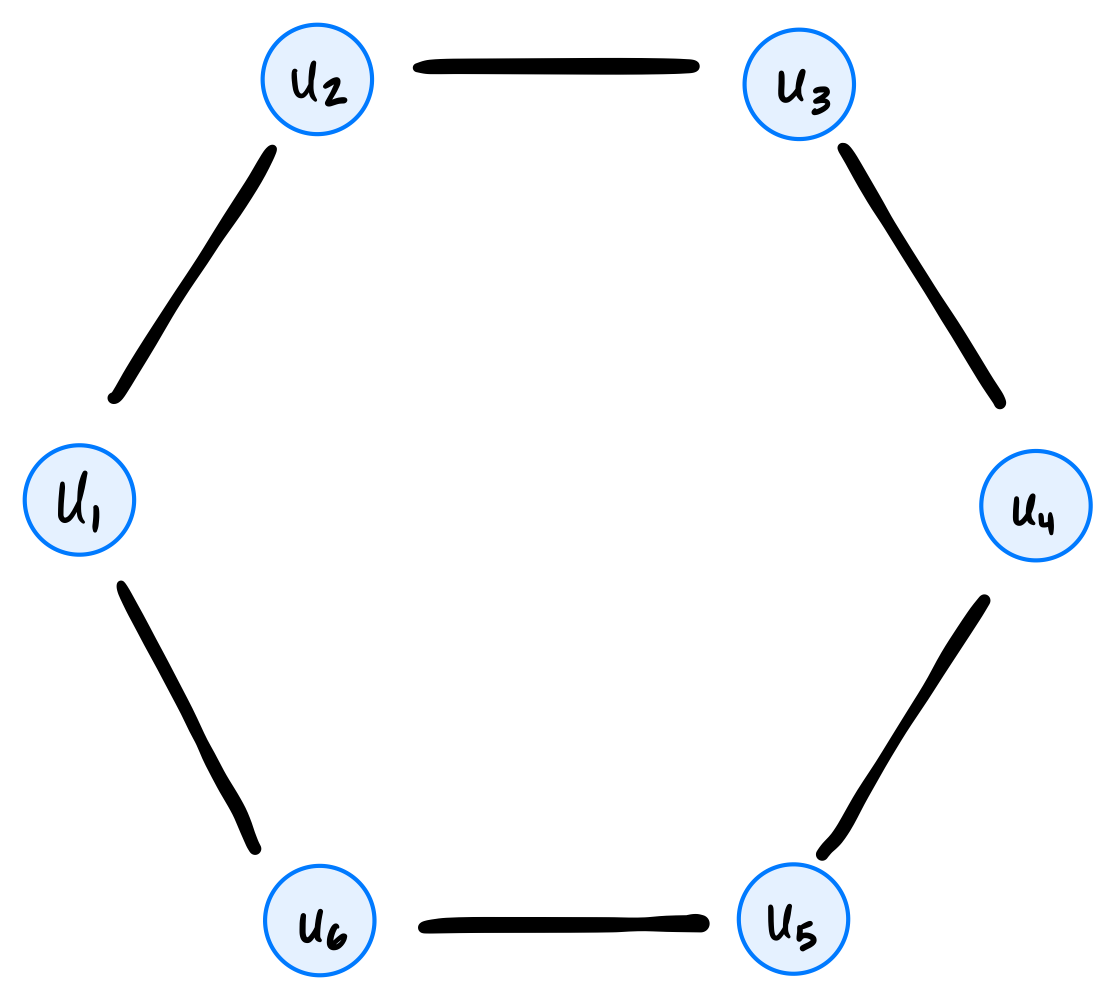
\includegraphics{./graph.png}

    What is the time complexity of breath-first search when run on a circle
    graph with $n$ nodes? State your answer as a function of $n$ using
    asymptotic notation.

    \begin{soln}
        $\Theta(n)$
    \end{soln}

\end{prob}
